\subsection{Inversion procedure}

\subsubsection{Sequantiual pseudo-inversion}

\todo{write this cleanly}

\paragraph{Truncation}

Intoduction of a new block can result in large fluctuating errors. This happens because the inverses are possible ill conditioned. Therefore the construction of the MPO should be stopped at a certain optimal order. Many different criteria can be tought of (and have been tried), but the most reliable method is as follows:

From the construction is can be seen that  the dimension of the new virtual level is at most $d^2$ times the dimension of the previous level. Depending on $\sigma_0$, the bond dimension is even lower.

The only parameter in the construction is $\sigma_0$ As can be seen in \cref{fig:sigman0}, mainly the construction for small values of $\beta$ get affected by the choice of $\sigma_0$.This can be seen in \cref{fig:sigman0}. A good tradeoff seems to be $ \sigma_0 = {10}^{-12}$. There is almost no precision loss vor small $\beta$, while for intermediate it performs optimal for intermediate $\beta$.

\begin{figure}
    \centering
    \begin{subfigure}{\textwidth}
        \centering
        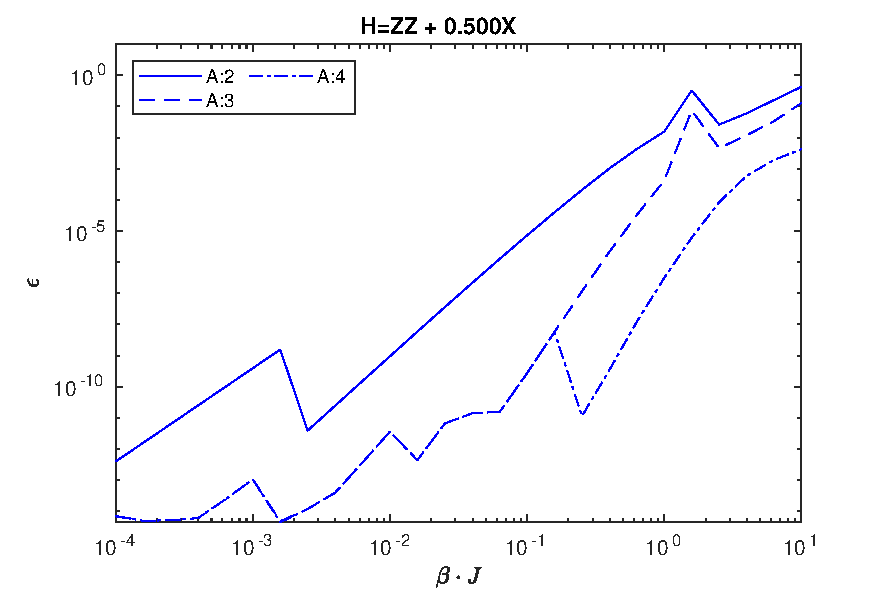
\includegraphics[width=0.8\linewidth]{Figuren/mpo_construction/sigm0/e10.pdf}
        \caption{ ${10}^{-10}$}
        \label{fig:sub1}
    \end{subfigure}%

    \begin{subfigure}{\textwidth}
        \centering
        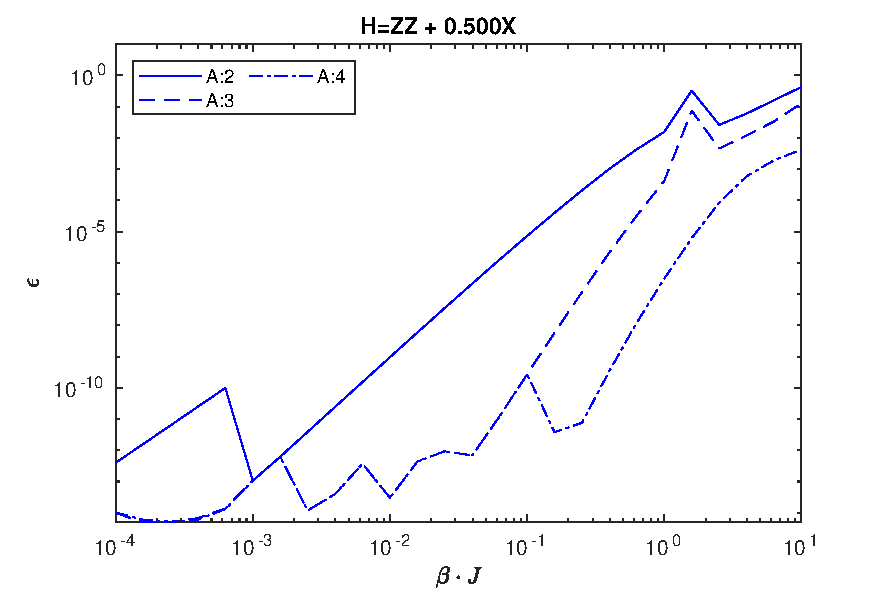
\includegraphics[width=0.8\linewidth]{Figuren/mpo_construction/sigm0/e11.pdf}
        \caption{${10}^{-11}$}
        \label{fig:sub2}
    \end{subfigure}
    \caption{A figure with two subfigures}
    \label{fig:sigman0}
\end{figure}

\begin{figure} \ContinuedFloat
    \centering
    \begin{subfigure}{\textwidth}
        \centering
        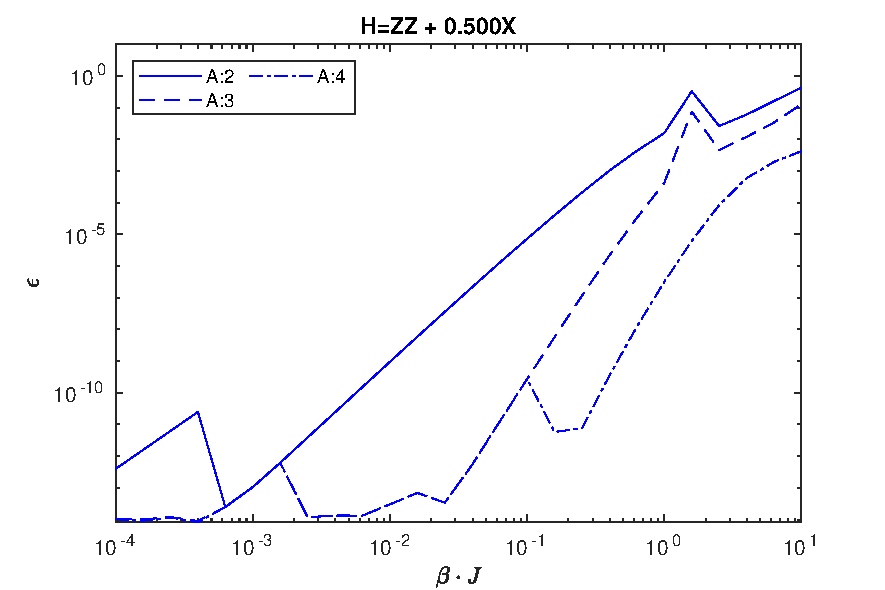
\includegraphics[width=0.8\linewidth]{Figuren/mpo_construction/sigm0/e12.pdf}
        \caption{ ${10}^{-12}$}
        \label{fig:sub1}
    \end{subfigure}%

    \begin{subfigure}{\textwidth}
        \centering
        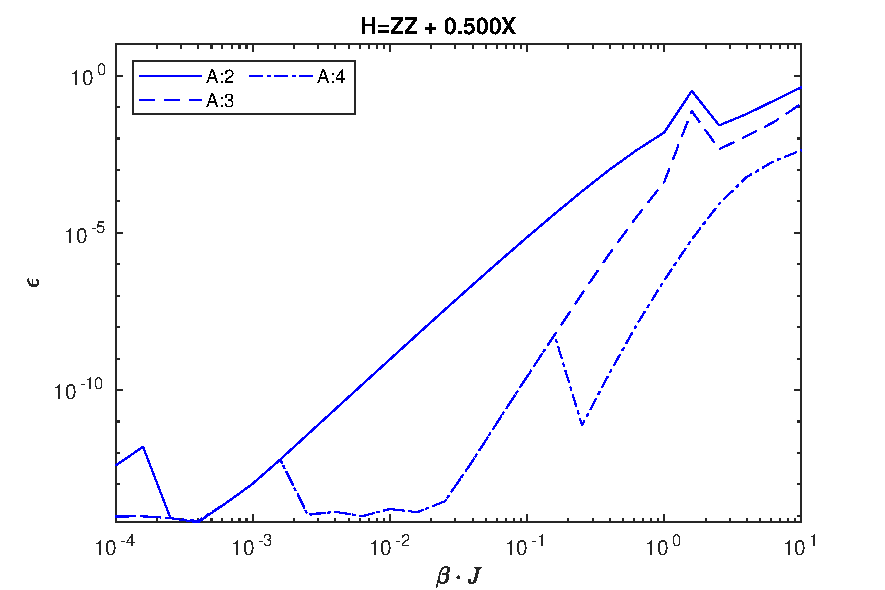
\includegraphics[width=0.8\linewidth]{Figuren/mpo_construction/sigm0/e13.pdf}
        \caption{${10}^{-13}$}
        \label{fig:sub2}
    \end{subfigure}
    \caption{A figure with two subfigures}
    \label{fig:sigman0}
\end{figure}

\begin{figure} \ContinuedFloat
    \centering
    \begin{subfigure}{\textwidth}
        \centering
        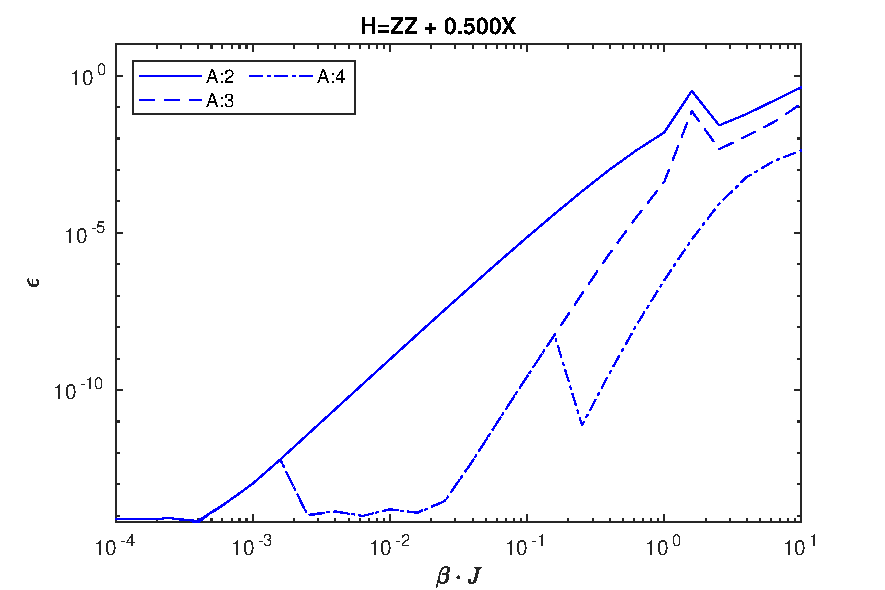
\includegraphics[width=0.8\linewidth]{Figuren/mpo_construction/sigm0/e14.pdf}
        \caption{ ${10}^{-14}$}
        \label{fig:sub1}
    \end{subfigure}%
    \caption{A figure with two subfigures}
    \label{fig:sigman0}
\end{figure}

\subsubsection{Full pseudo-inversion}

\subsection{Models}

\subsubsection{Ising}

The first model used to benchmark the different types of MPO's is the transversal ising model. For type A the $\epsilon$ increases with
$\beta$. As expected, the relative error decreases with increasing order.

The behaviour of type B is more chaotic. The error increases no longer monotonously. For small values of $\beta$, the order is truncated.

For type 5 \cref{bench:ising5}, there is a consitent improvement over type B. \todo{larger orders need reimplementation (non matrix based)}

\begin{figure}[H]
    \center
    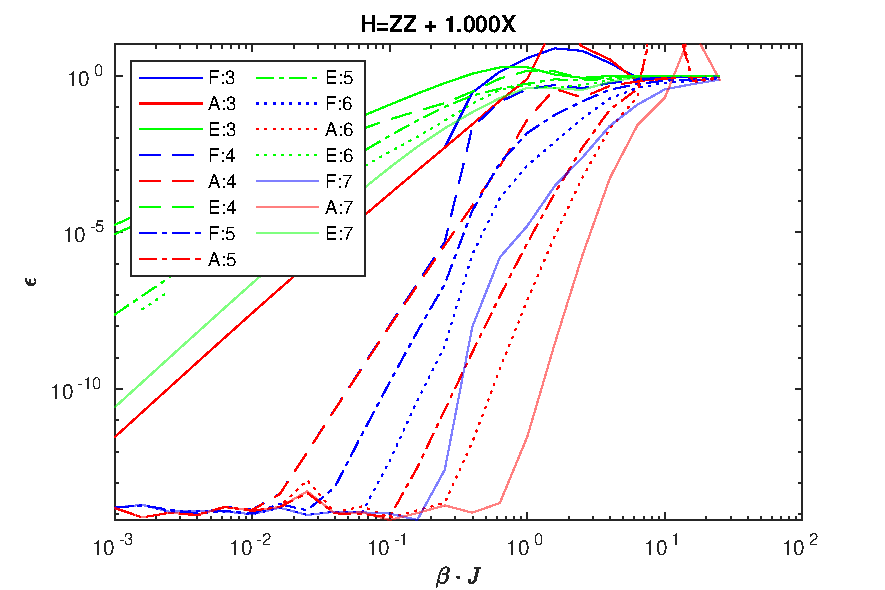
\includegraphics[width=\textwidth]{Figuren/benchmarking/t_ising.pdf}
    \caption{Comparison type A and B for Transversal Ising}
    \label{fig:benchmark:tising}
\end{figure}

\begin{figure}[H]
    \center
    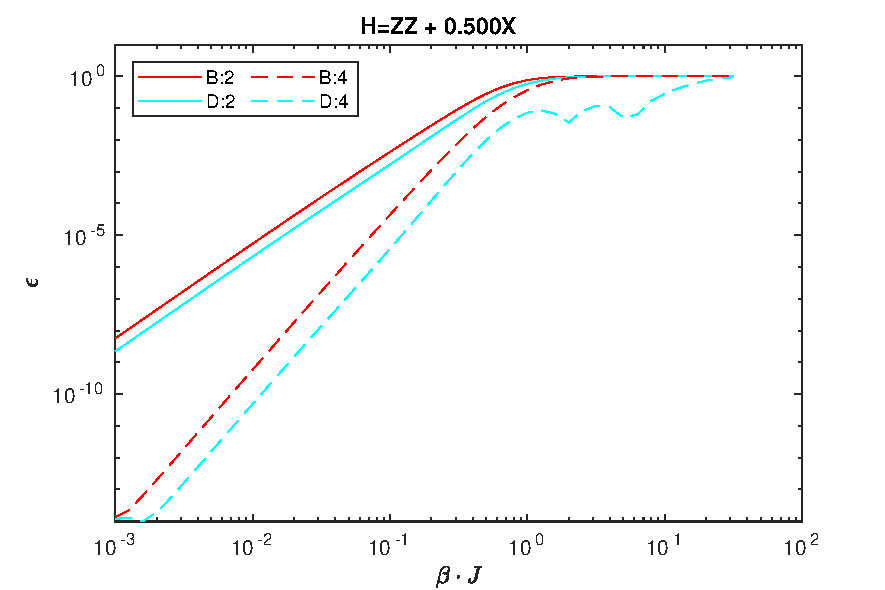
\includegraphics[width=\textwidth]{Figuren/benchmarking/type5/ising.pdf}
    \caption{Comparison type C and B for Transversal Ising}
    \label{bench:ising5}
\end{figure}

\subsubsection{Heisenberg}

For the Heisenberg model, type A is also an improvement over type B. For large values of $\beta$, increasing the order does not help. Type 5 \cref{bench:type5heis} is more promising, but higher orders require to much memory to simulate.

\begin{figure}[H]
    \center
    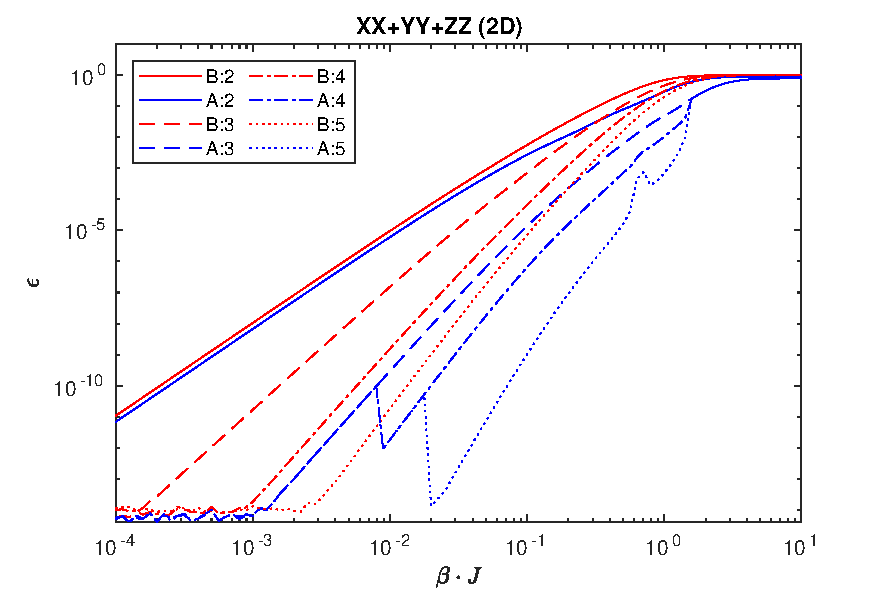
\includegraphics[width=\textwidth]{Figuren/benchmarking/heis_XXX.pdf}
    \caption{Comparison type A and B for Heisenberg}
    \label{fig:benchmark:Heisenberg}
\end{figure}

\begin{figure}[H]
    \center
    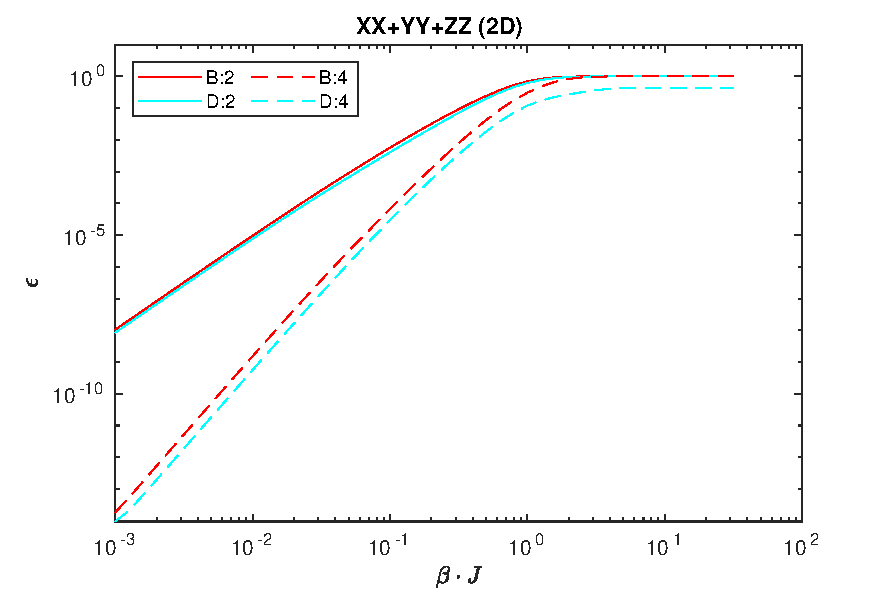
\includegraphics[width=\textwidth]{Figuren/benchmarking/type5/heis.pdf}
    \caption{Comparison type C and B for Heisenberg}
    \label{bench:type5heis}
\end{figure}

\begin{figure}[H]
    \center
    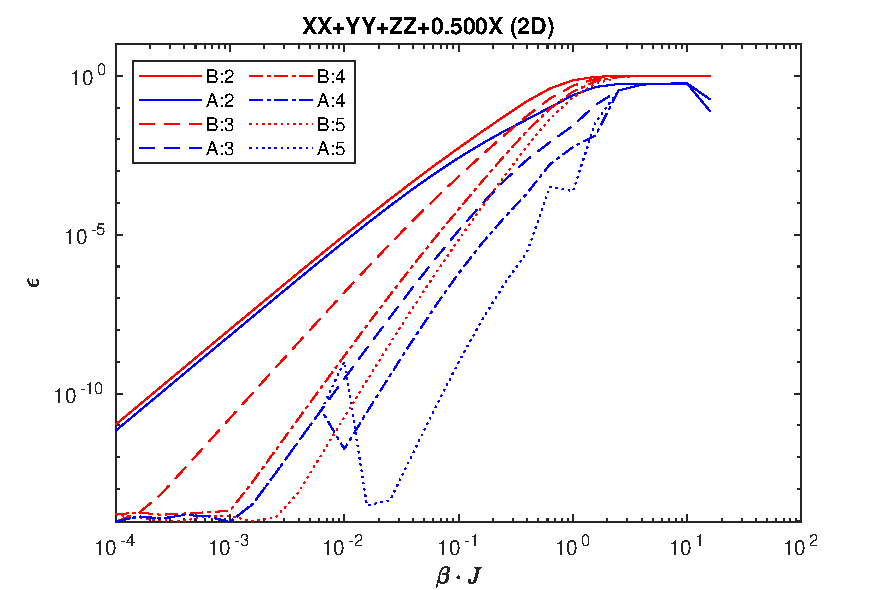
\includegraphics[width=\textwidth]{Figuren/benchmarking/t_heis_XXX.pdf}
    \caption{transversal XXX}
    \label{fig:benchmark:tHeisenberg}
\end{figure}

\todo{run with M=11}

\subsubsection{Random}

To give a representative overview for random hamiltonians, several simulations were run. The single site and nearest neighbourgh hamiltonians are generated by making hermitian matrices with random real and complex numbers between -1 and 1. In order to compare the different graphs, the engergy scale is set such that the norm of the 2 site hamiltonian is 1.

Clearly, the performance of type B is almost independent on the chosen random variables. For type A there is more variation. Still, A performs almost always better than B. For some random models, such as \cref{benchmark:rand2}, the order is truncated at low order for high temperatures (see peak at $\beta J \approxeq 4$). It6s unclear why this behaviour emerges. Manually overinding the sefagaurd machanism

\todo{blabla}

\begin{figure}[H]
    \begin{subfigure}[]{\textwidth}
        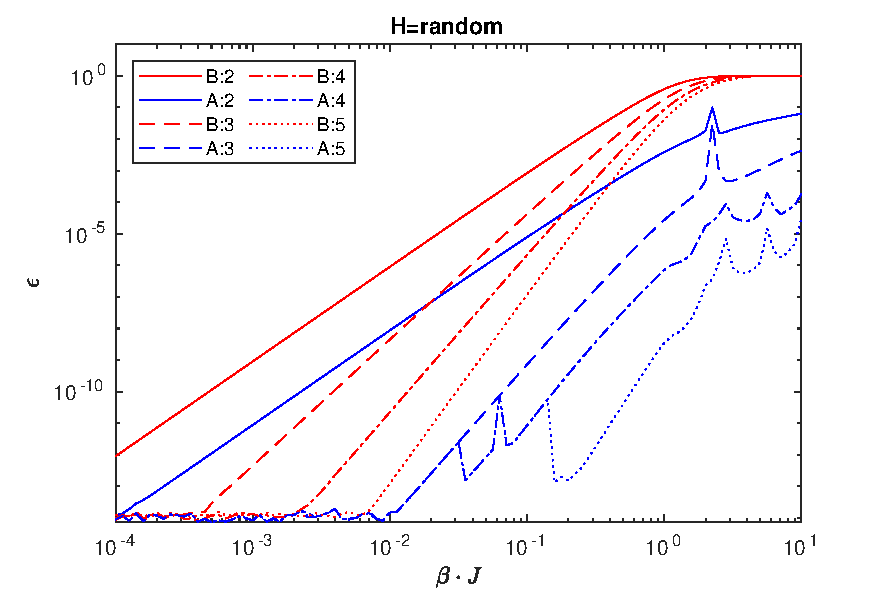
\includegraphics[width=\textwidth]{Figuren/benchmarking/rand_01.pdf}
        \subcaption{test}
    \end{subfigure}

    \medskip

    \begin{subfigure}[]{\textwidth}
        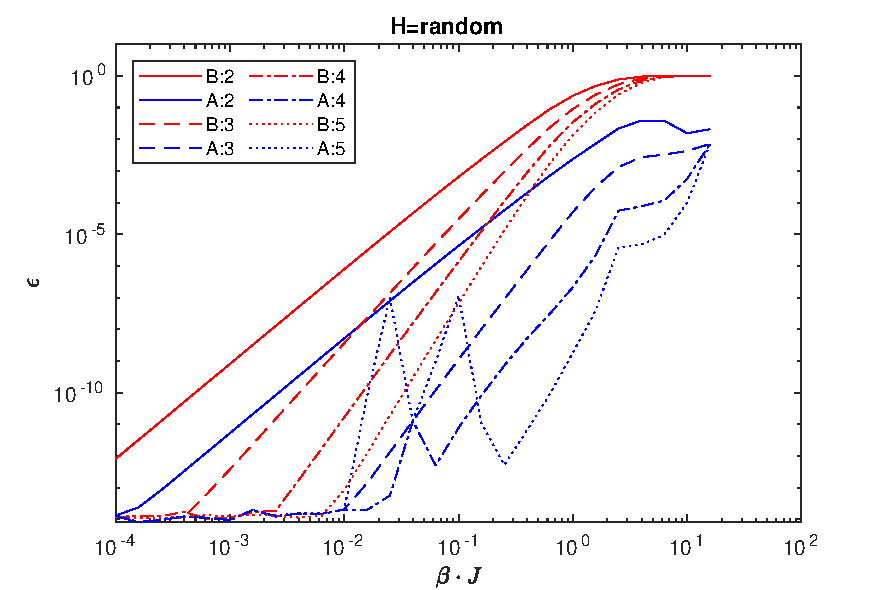
\includegraphics[width=\textwidth]{Figuren/benchmarking/rand_02.pdf}
        \subcaption{test}
        \label{benchmark:rand2}
    \end{subfigure}

    \caption{test }
\end{figure}

\begin{figure}[H]\ContinuedFloat
    \begin{subfigure}[]{\textwidth}
        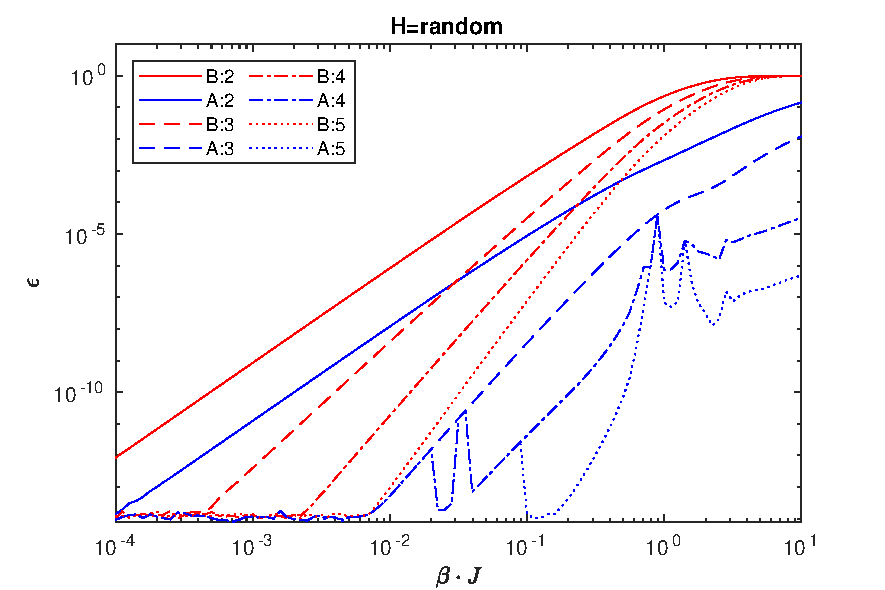
\includegraphics[width=\textwidth]{Figuren/benchmarking/rand_03.pdf}
        \subcaption{test}
    \end{subfigure}

    \begin{subfigure}[]{\textwidth}
        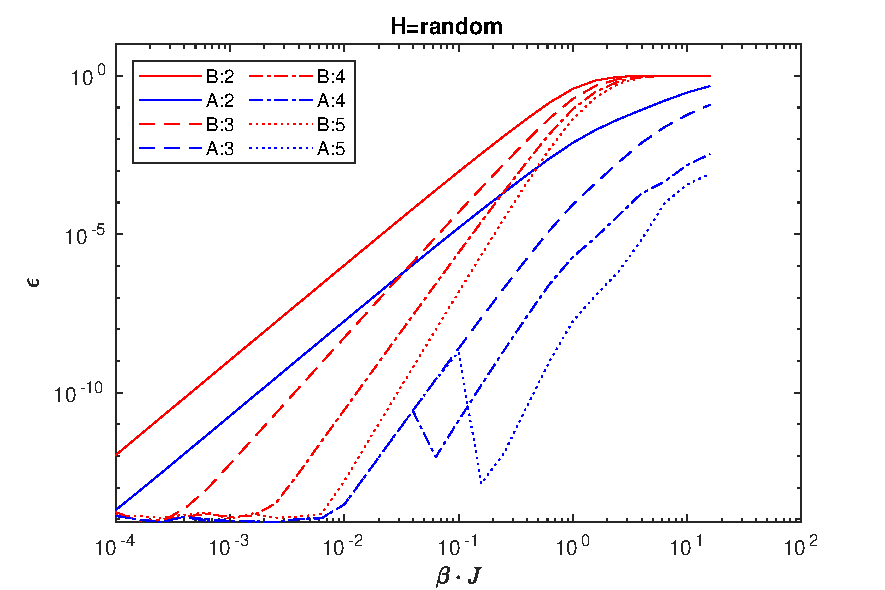
\includegraphics[width=\textwidth]{Figuren/benchmarking/rand_04.pdf}
        \subcaption{test}
    \end{subfigure}
    \caption{test (cont.) }
    \label{fig:benchmark:Random}
\end{figure}

Also here type D improve the results of type B. For high $\beta$ truncation seems necessary. \todo{nog niet klaar}

\begin{figure}[H]
    \center
    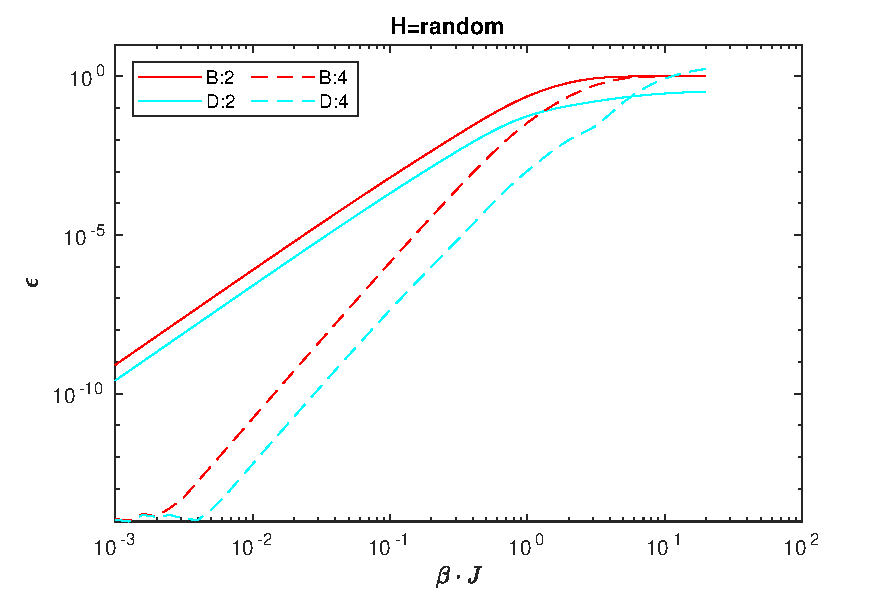
\includegraphics[width=\textwidth]{Figuren/benchmarking/type5/ranodm.pdf}
    \caption{Comparison type C and B for random Hamiltonian}
\end{figure}

